\documentclass[a4paper,11pt]{article}
\usepackage{geometry}
\geometry{margin=1in, headheight=15pt}
\usepackage{amsmath}
\usepackage{amssymb}
\usepackage{mathtools}
\usepackage{graphicx}
\usepackage{xcolor}
\definecolor{blue3}{RGB}{0,0,180}
\definecolor{green3}{RGB}{0,120,0}
\definecolor{orange3}{RGB}{200,100,0}
\usepackage{siunitx}
\sisetup{detect-all}
\usepackage[colorlinks=true,linkcolor=blue3,citecolor=blue3,urlcolor=blue3]{hyperref}
\usepackage{cleveref}
\usepackage{tcolorbox}
\tcbuselibrary{skins,breakable}
\newtcolorbox{derivationbox}[1][]{colback=blue!10,colframe=blue3,coltitle=blue3,title={Derivation:},fonttitle=\bfseries,#1}
\newtcolorbox{resultbox}[1][]{colback=green!10,colframe=green3,coltitle=green3,title={Result Summary:},fonttitle=\bfseries,#1}
\newtcolorbox{keyformulabox}[1][]{colback=orange!10,colframe=orange3,coltitle=orange3,title={Key Formula:},fonttitle=\bfseries,#1}
\usepackage{booktabs}
\usepackage{enumitem}
\usepackage{tikz}
\usetikzlibrary{arrows.meta, decorations.markings}
\newcommand{\khat}{\hat{k}}
\newcommand{\chat}{\hat{c}}
\newcommand{\yhat}{\hat{y}}

\title{\textbf{Ramsey--Cass--Koopmans Model}\\
       \large Lecture 2 Cheatsheet --- 14E022 Macroeconomics I}
\author{BSE --- Alessandro Ferrari}
\date{2026}

\begin{document}

\maketitle
\tableofcontents
\newpage

%%%%%%%%%%%%%%%%%%%%%%%%%%%%%%%%%%%%%%%%%%%%%%%%%%%%%%%%%%%%%
\section{Notation and Definitions}
%%%%%%%%%%%%%%%%%%%%%%%%%%%%%%%%%%%%%%%%%%%%%%%%%%%%%%%%%%%%%

\begin{center}
\begin{tabular}{lll}
\toprule
\textbf{Symbol} & \textbf{Definition} & \textbf{Units / Notes} \\
\midrule
$K_t$ & Aggregate capital stock & Level \\
$L_t = N_t$ & Labor / population & Level \\
$C_t$, $c_t$ & Aggregate / per-worker consumption & $c_t = C_t/L_t$ \\
$k_t$ & Per-worker capital & $k_t = K_t/L_t$ \\
$\khat_t$ & Per-effective-worker capital & $\khat_t = K_t/(B_t L_t)$ \\
$\chat_t$ & Per-effective-worker consumption & $\chat_t = C_t/(B_t L_t)$ \\
$\yhat_t$ & Per-effective-worker output & $\yhat_t = f(\khat_t)$ \\
$a_t$ & Per-worker assets (= $k_t$ in eq.) & \\
$n$ & Population growth rate & $\dot{N}/N = n$ \\
$x$ & Rate of labor-augmenting tech.\ progress & $\dot{B}/B = x$ \\
$\delta$ & Capital depreciation rate & \\
$\rho$ & Household rate of time preference & $\rho > 0$ \\
$\sigma$ & Inverse elasticity of intertemporal sub. & $\sigma > 0$ \\
$\alpha$ & Capital share in Cobb-Douglas & $0 < \alpha < 1$ \\
$\nu_t$ & Current-value co-state (shadow price) & \\
$r_t$ & Rental rate of capital & $r_t = f'(k_t) - \delta$ \\
$w_t$ & Wage & $w_t = f(k_t) - k_t f'(k_t)$ \\
\bottomrule
\end{tabular}
\end{center}

\subsection*{Key Transformations}
\[
  \khat_t = \frac{k_t}{B_t}, \qquad
  \chat_t = \frac{c_t}{B_t}, \qquad
  \yhat_t = \frac{y_t}{B_t} = f(\khat_t).
\]
Growth rates obey $\gamma_x \equiv \dot{x}/x$. For a hat variable $\hat{z} = z/B$:
\[
  \gamma_{\hat{z}} = \gamma_z - x.
\]

%%%%%%%%%%%%%%%%%%%%%%%%%%%%%%%%%%%%%%%%%%%%%%%%%%%%%%%%%%%%%
\section{Environment and Welfare Theorems}
%%%%%%%%%%%%%%%%%%%%%%%%%%%%%%%%%%%%%%%%%%%%%%%%%%%%%%%%%%%%%

\subsection*{Demographics and Technology}
\[
  N_t = N_0 \, e^{nt}, \qquad B_t = B_0 \, e^{xt} \quad \text{(labor-augmenting; Uzawa theorem)}.
\]
Effective labor: $A_t = B_t N_t$.

\subsection*{Preferences}
The representative household has $N_0 e^{nt}$ members and maximizes
\[
  U_0 = \int_0^{\infty} u(c_t)\, e^{-(\rho - n)t}\, dt,
\]
where $u(c_t)$ is instantaneous utility, $\rho - n > 0$ is required for convergence.

\subsection*{Welfare Theorems}
Under the standard assumptions (no externalities, complete markets, no distortions), the \textbf{First and Second Welfare Theorems} apply:
\begin{itemize}[leftmargin=*]
  \item The competitive equilibrium allocation is Pareto optimal.
  \item The social planner's problem and the decentralized equilibrium yield \emph{identical} allocations.
  \item Consequence: we can solve either problem and obtain the same dynamics.
\end{itemize}

%%%%%%%%%%%%%%%%%%%%%%%%%%%%%%%%%%%%%%%%%%%%%%%%%%%%%%%%%%%%%
\section{Household Problem}
%%%%%%%%%%%%%%%%%%%%%%%%%%%%%%%%%%%%%%%%%%%%%%%%%%%%%%%%%%%%%

\subsection*{Budget Constraint}
In per-worker terms, assets $a_t$ evolve as:
\[
  \dot{a}_t = w_t + r_t a_t - c_t - n a_t,
\]
or equivalently,
\[
  \dot{a}_t + n a_t = w_t + r_t a_t - c_t. \tag{BC}
\]
In market clearing, $a_t = k_t$.

\subsection*{No-Ponzi Condition}
\[
  \lim_{t \to \infty} a_t \exp\!\left(-\int_0^t \bigl(r(s) - n\bigr)\, ds\right) \geq 0. \tag{NPC}
\]
This prevents households from rolling over debt forever (dying in debt). Combined with the optimality condition (TVC), this holds with equality in the optimum.

\subsection*{Transversality Condition (TVC)}
\[
  \lim_{t \to \infty} \nu_t \, a_t = 0. \tag{TVC}
\]
where $\nu_t$ is the shadow price of assets in the current-value Hamiltonian. The TVC ensures the household does not leave unconsumed wealth at infinity.

%%%%%%%%%%%%%%%%%%%%%%%%%%%%%%%%%%%%%%%%%%%%%%%%%%%%%%%%%%%%%
\section{Hamiltonian Derivation}
%%%%%%%%%%%%%%%%%%%%%%%%%%%%%%%%%%%%%%%%%%%%%%%%%%%%%%%%%%%%%

\subsection*{Setup}
\begin{itemize}[leftmargin=*]
  \item \textbf{Control variable:} $c_t$ (consumption).
  \item \textbf{State variable:} $a_t$ (assets / capital).
  \item \textbf{Co-state variable:} $\nu_t$ (shadow price of assets).
\end{itemize}

\subsection*{Present-Value Hamiltonian}
\[
  \mathcal{J}(c_t,\, a_t,\, \nu_t,\, t)
  = u(c_t)\, e^{-(\rho - n)t}
    + \nu_t \Bigl[w_t + (r_t - n)\, a_t - c_t\Bigr]. \tag{PVH}
\]

\begin{derivationbox}[title={Deriving the Euler Equation from FOCs}]
\textbf{FOC 1 --- control variable:}
\[
  \frac{\partial \mathcal{J}}{\partial c_t} = 0
  \implies \nu_t = u_c(c_t)\, e^{-(\rho - n)t}. \tag{F1}
\]

\textbf{FOC 2 --- co-state equation:}
\[
  \frac{\partial \mathcal{J}}{\partial a_t} = -\dot{\nu}_t
  \implies \dot{\nu}_t = -(r_t - n)\,\nu_t. \tag{F2}
\]

\textbf{FOC 3 --- state equation (reproduced):}
\[
  \frac{\partial \mathcal{J}}{\partial \nu_t} = \dot{a}_t
  \implies \dot{a}_t = w_t + (r_t - n)\,a_t - c_t. \tag{F3}
\]

\textbf{Euler equation from F1 and F2:}\\[4pt]
Take logs of (F1): $\ln \nu_t = \ln u_c(c_t) - (\rho - n)t$.

Differentiate with respect to $t$:
\[
  \frac{\dot{\nu}_t}{\nu_t} = \frac{u_{cc}(c_t)\, \dot{c}_t}{u_c(c_t)} - (\rho - n).
\]
Substitute (F2) for $\dot{\nu}_t/\nu_t = -(r_t - n)$:
\[
  -(r_t - n) = \frac{u_{cc}(c_t)\, \dot{c}_t}{u_c(c_t)} - (\rho - n).
\]
Rearrange:
\[
  \frac{\dot{c}_t}{c_t}
  = -\frac{u_c(c_t)}{u_{cc}(c_t)\, c_t}\,(r_t - \rho).
\]
Define the \textbf{elasticity of intertemporal substitution} $\varepsilon(c) \equiv -u_c/(u_{cc} c)$:
\[
  \boxed{\frac{\dot{c}_t}{c_t} = \varepsilon(c_t)\,(r_t - \rho).}
\]
\end{derivationbox}

%%%%%%%%%%%%%%%%%%%%%%%%%%%%%%%%%%%%%%%%%%%%%%%%%%%%%%%%%%%%%
\section{CRRA Utility and the Euler Equation}
%%%%%%%%%%%%%%%%%%%%%%%%%%%%%%%%%%%%%%%%%%%%%%%%%%%%%%%%%%%%%

\subsection*{CRRA Functional Form}
\[
  u(c) = \frac{c^{1-\sigma} - 1}{1 - \sigma}, \qquad \sigma > 0, \; \sigma \neq 1.
\]
For $\sigma = 1$: $u(c) = \ln c$ (log utility).

Properties: $u_c = c^{-\sigma}$, $u_{cc} = -\sigma c^{-\sigma - 1}$, so
\[
  \varepsilon(c) = -\frac{u_c}{u_{cc}\, c} = \frac{1}{\sigma}.
\]

\subsection*{Euler Equation (CRRA)}
\begin{resultbox}
\[
  \frac{\dot{c}_t}{c_t} = \frac{1}{\sigma}\,(r_t - \rho).
\]
Interpretation: consumption grows fast when the return to saving $r_t$ exceeds the discount rate $\rho$. $\sigma$ governs how strongly households respond to interest rate incentives.
\end{resultbox}

\subsection*{In Per-Effective-Worker Terms}
Since $\chat = c/B$ and $\dot{B}/B = x$:
\[
  \frac{\dot{\chat}}{\chat} = \frac{\dot{c}}{c} - x
  = \frac{1}{\sigma}(r_t - \rho) - x.
\]
Using $r_t = f'(\khat) - \delta$:
\begin{keyformulabox}
\[
  \frac{\dot{\chat}}{\chat}
  = \frac{1}{\sigma}\bigl[f'(\khat_t) - \delta - \rho - \sigma x\bigr]. \tag{Euler-hat}
\]
\end{keyformulabox}

%%%%%%%%%%%%%%%%%%%%%%%%%%%%%%%%%%%%%%%%%%%%%%%%%%%%%%%%%%%%%
\section{Firm Problem}
%%%%%%%%%%%%%%%%%%%%%%%%%%%%%%%%%%%%%%%%%%%%%%%%%%%%%%%%%%%%%

\subsection*{Technology}
Firms have CRS production: $Y_t = F(K_t, B_t L_t)$, or in intensive form $\yhat = f(\khat)$ where $f$ is concave, $f(0) = 0$, Inada conditions hold.

\subsection*{Profit Maximization (competitive firms)}
Firms rent capital and hire labor each period:
\[
  \max_{K,L} \; F(K, BL) - r_t K - w_t L.
\]
FOCs (using Euler's theorem for CRS):
\[
  r_t = F_K = f'(\khat_t), \qquad
  w_t = F_{BL} \cdot B_t = B_t\bigl[f(\khat_t) - \khat_t f'(\khat_t)\bigr].
\]
Note: in equilibrium $r_t = f'(\khat) - \delta$ (net of depreciation).

\subsection*{Cobb-Douglas Special Case}
\[
  f(\khat) = \khat^{\alpha}, \quad
  f'(\khat) = \alpha \khat^{\alpha - 1}, \quad
  f(\khat) - \khat f'(\khat) = (1-\alpha)\khat^{\alpha}.
\]

%%%%%%%%%%%%%%%%%%%%%%%%%%%%%%%%%%%%%%%%%%%%%%%%%%%%%%%%%%%%%
\section{Dynamic System}
%%%%%%%%%%%%%%%%%%%%%%%%%%%%%%%%%%%%%%%%%%%%%%%%%%%%%%%%%%%%%

The equilibrium is fully described by two ODEs in $(\khat_t, \chat_t)$:

\begin{keyformulabox}[title={Two-ODE System}]
\begin{align*}
  \dot{\khat}_t &= f(\khat_t) - \chat_t - (n + x + \delta)\,\khat_t,
  \tag{K-dot} \\[6pt]
  \frac{\dot{\chat}_t}{\chat_t} &= \frac{1}{\sigma}\bigl[f'(\khat_t) - \delta - \rho - \sigma x\bigr].
  \tag{C-dot}
\end{align*}
\end{keyformulabox}

\subsection*{Derivation of (K-dot)}
The aggregate resource constraint is $\dot{K} = Y - C - \delta K$.
Divide by $B L$, use $(\dot{K}/(BL)) = \dot{\khat} + (n+x)\khat$:
\[
  \dot{\khat} = f(\khat) - \chat - (n+x+\delta)\khat.
\]

\subsection*{Boundary Conditions}
\begin{itemize}[leftmargin=*]
  \item Initial condition: $\khat_0$ given (predetermined state).
  \item TVC / No-Ponzi at infinity: pins down the initial value of $\chat_0$ (the \emph{jump} variable).
\end{itemize}

%%%%%%%%%%%%%%%%%%%%%%%%%%%%%%%%%%%%%%%%%%%%%%%%%%%%%%%%%%%%%
\section{Steady State and Modified Golden Rule}
%%%%%%%%%%%%%%%%%%%%%%%%%%%%%%%%%%%%%%%%%%%%%%%%%%%%%%%%%%%%%

\subsection*{Conditions}
Set $\dot{\khat} = 0$ and $\dot{\chat} = 0$:

\begin{resultbox}[title={Steady State Equations}]
\begin{align*}
  \dot{\chat}^* = 0 &\implies \boxed{f'(\khat^*) = \delta + \rho + \sigma x}
  & \text{(Modified Golden Rule)} \tag{MGR} \\[4pt]
  \dot{\khat}^* = 0 &\implies \chat^* = f(\khat^*) - (n+x+\delta)\khat^*
  & \text{(resource balance)}
\end{align*}
\end{resultbox}

The Modified Golden Rule (MGR) pins down $\khat^*$ \emph{independently of $n$}, unlike the Solow model.

\subsection*{Cobb-Douglas Closed Forms}
With $f(\khat) = \khat^\alpha$, from MGR: $\alpha (\khat^*)^{\alpha-1} = \delta + \rho + \sigma x$, so
\[
  \khat^* = \left(\frac{\alpha}{\delta + \rho + \sigma x}\right)^{1/(1-\alpha)}, \qquad
  \yhat^* = \left(\frac{\alpha}{\delta + \rho + \sigma x}\right)^{\alpha/(1-\alpha)}.
\]

\subsection*{Steady-State Interest Rate and Savings Rate}
\[
  r^* = f'(\khat^*) - \delta = \rho + \sigma x.
\]
\[
  s^* = \frac{(n+x+\delta)\khat^*}{f(\khat^*)}
      = \frac{\alpha(n+x+\delta)}{\delta + \rho + \sigma x + n}.
\]
With Cobb-Douglas: $s^* = \frac{\alpha(n+x+\delta)}{\delta + \rho + \sigma x} \cdot \frac{\khat^*}{yhat^*} \cdot \frac{1}{\khat^*} \approx \frac{\alpha(n+x+\delta)}{\rho + \sigma x + \delta}$, which is \emph{less than} the Solow savings rate $s = \alpha$ at the Golden Rule.

\subsection*{TVC Implication: No Dynamic Inefficiency}
The TVC requires:
\[
  n + (1-\sigma)x - \rho < 0.
\]
This ensures $\khat^* < \khat^*_{\text{Golden Rule}}$, i.e., the economy does \emph{not} over-accumulate capital. Dynamic inefficiency is ruled out by assumption; the Ramsey model satisfies the Modified (not the standard) Golden Rule.

Recall: Golden Rule maximizes $\chat$, requiring $f'(\khat_g) = n + x + \delta$. Since $\rho + \sigma x > 0$, we have $f'(\khat^*) > f'(\khat_g)$, hence $\khat^* < \khat_g$.

%%%%%%%%%%%%%%%%%%%%%%%%%%%%%%%%%%%%%%%%%%%%%%%%%%%%%%%%%%%%%
\section{Phase Diagram}
%%%%%%%%%%%%%%%%%%%%%%%%%%%%%%%%%%%%%%%%%%%%%%%%%%%%%%%%%%%%%

\subsection*{Loci and Dynamics}
\begin{itemize}[leftmargin=*]
  \item $\dot{\chat} = 0$: vertical line at $\khat = \khat^*$ (from MGR).
  \item $\dot{\khat} = 0$: inverted-U curve $\chat = f(\khat) - (n+x+\delta)\khat$; peaks at Golden Rule $\khat_g$ where $f'(\khat_g) = n+x+\delta$.
  \item Above $\dot{\khat}=0$: $\dot{\khat} < 0$ (capital declines). Below: $\dot{\khat} > 0$.
  \item Right of $\dot{\chat}=0$: $\dot{\chat} < 0$ (consumption declines). Left: $\dot{\chat} > 0$.
\end{itemize}

\subsection*{Saddle-Path Stability}
The steady state is a \textbf{saddle point}: one stable and one unstable manifold. The \textbf{saddle path} (stable arm) is the unique trajectory converging to $(\khat^*, \chat^*)$. The initial value $\chat_0$ is chosen to place the economy on the saddle path.

\begin{center}
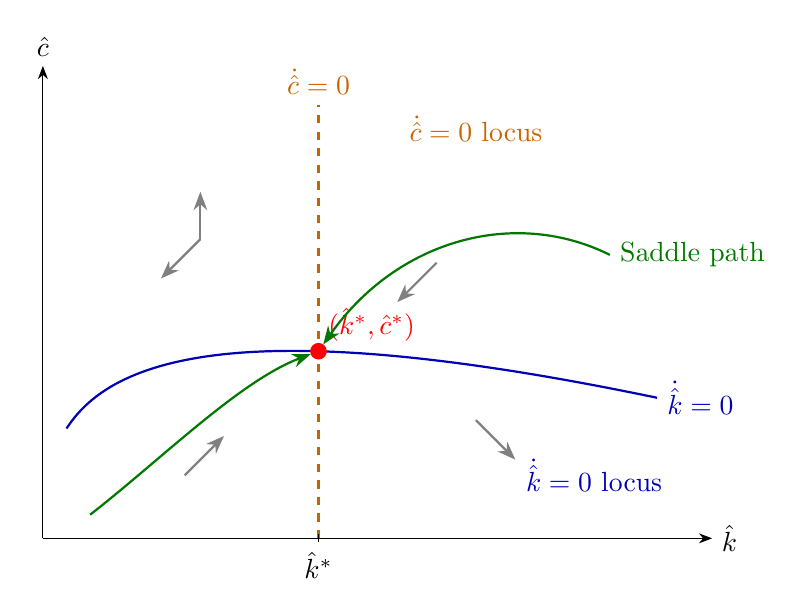
\begin{tikzpicture}[scale=1.0, >=Stealth]
  % Axes
  \draw[->] (0,0) -- (8.5,0) node[right] {$\khat$};
  \draw[->] (0,0) -- (0,6) node[above] {$\chat$};

  % kdot=0 locus: inverted U, peaks near k=4
  \draw[thick, blue3, domain=0.3:7.8, samples=120]
    plot (\x, {2.5*\x^0.4 - 0.5*\x}) node[right] {$\dot{\khat}=0$};

  % cdot=0: vertical line at khat*=3.5
  \draw[thick, orange3, dashed] (3.5,0) -- (3.5,5.5)
    node[above] {$\dot{\chat}=0$};

  % Steady state point
  \coordinate (SS) at (3.5, {2.5*3.5^0.4 - 0.5*3.5});
  \fill[red] (SS) circle (3pt) node[above right] {$(\khat^*,\chat^*)$};

  % Saddle path: concave curve from bottom-left toward SS
  \draw[thick, green3, ->, shorten >=3pt]
    (0.6, 0.3) .. controls (1.5, 1.0) and (2.5, 2.0) .. (SS);
  \draw[thick, green3, <-, shorten <=3pt]
    (SS) .. controls (4.5, 3.8) and (6.0, 4.2) .. (7.2, 3.6)
    node[right] {\color{green3}Saddle path};

  % Directional arrows in quadrants
  % Quadrant NE: khat > khat*, chat above kdot=0: khat-dot<0, cdot<0
  \draw[->, thick, gray] (5.0, 3.5) -- (4.5, 3.0);
  % Quadrant NW: khat < khat*, chat above kdot=0: khat-dot<0, cdot>0
  \draw[->, thick, gray] (2.0, 3.8) -- (2.0, 4.4);
  \draw[->, thick, gray] (2.0, 3.8) -- (1.5, 3.3);
  % Quadrant SE: khat > khat*, chat below kdot=0: khat-dot>0, cdot<0
  \draw[->, thick, gray] (5.5, 1.5) -- (6.0, 1.0);
  % Quadrant SW: khat < khat*, chat below kdot=0: khat-dot>0, cdot>0
  \draw[->, thick, gray] (1.8, 0.8) -- (2.3, 1.3);

  % Labels for axes ticks
  \draw (3.5, 0.05) -- (3.5,-0.05) node[below] {$\khat^*$};

  % Legend
  \node[blue3] at (7.0, 0.8) {$\dot{\khat}=0$ locus};
  \node[orange3] at (5.5, 5.2) {$\dot{\chat}=0$ locus};
\end{tikzpicture}
\end{center}

%%%%%%%%%%%%%%%%%%%%%%%%%%%%%%%%%%%%%%%%%%%%%%%%%%%%%%%%%%%%%
\section{Comparative Statics}
%%%%%%%%%%%%%%%%%%%%%%%%%%%%%%%%%%%%%%%%%%%%%%%%%%%%%%%%%%%%%

\begin{center}
\begin{tabular}{lcccc}
\toprule
\textbf{Parameter} & $\Delta$ & \textbf{Affected locus} & $\khat^*$ & $\chat^*$ \\
\midrule
$\rho$ (impatience) $\uparrow$ & $+$ & $\dot{\chat}=0$ shifts left & $\downarrow$ & $\downarrow$ \\
$\sigma$ (risk aversion) $\uparrow$ & $+$ & $\dot{\chat}=0$ shifts left (if $x>0$) & $\downarrow$ & $\downarrow$ \\
$\delta$ (depreciation) $\uparrow$ & $+$ & $\dot{\chat}=0$ shifts left; $\dot{\khat}=0$ shifts down & $\downarrow$ & $\downarrow$ \\
$n$ (pop.\ growth) $\uparrow$ & $+$ & $\dot{\khat}=0$ shifts down & \emph{none} & $\downarrow$ \\
$x$ (tech.\ progress) $\uparrow$ & $+$ & $\dot{\chat}=0$ shifts left; $\dot{\khat}=0$ shifts down & $\downarrow$ & --- \\
$\alpha$ (capital share) $\uparrow$ & $+$ & Both loci shift & $\uparrow$ & $\uparrow$ \\
\bottomrule
\end{tabular}
\end{center}

\subsection*{Effect of an Increase in $\rho$}
\begin{enumerate}[leftmargin=*]
  \item $\dot{\chat}=0$ locus shifts \emph{left} (households want to consume more now).
  \item Instantaneous jump up in $\chat_0$ (control variable can jump).
  \item $\khat$ falls over transition (more consumption, less investment).
  \item New steady state: lower $\khat^*$ and $\chat^*$.
\end{enumerate}
Key: \emph{$n$ does not affect $\khat^*$}, unlike the Solow model.

\subsection*{Effect of $n$ on Steady State}
From MGR: $f'(\khat^*) = \delta + \rho + \sigma x$ --- no $n$ appears! So $\khat^*$ is independent of $n$. However, $\chat^* = f(\khat^*) - (n+x+\delta)\khat^*$ falls as $n$ rises (more workers dilute capital).

%%%%%%%%%%%%%%%%%%%%%%%%%%%%%%%%%%%%%%%%%%%%%%%%%%%%%%%%%%%%%
\section{Comparison to Solow Model}
%%%%%%%%%%%%%%%%%%%%%%%%%%%%%%%%%%%%%%%%%%%%%%%%%%%%%%%%%%%%%

\begin{center}
\begin{tabular}{lll}
\toprule
\textbf{Feature} & \textbf{Solow} & \textbf{Ramsey} \\
\midrule
Savings rate $s$ & Exogenous constant & Endogenous (optimized) \\
Steady state $\khat^*$ & $f(\khat^*) = (n+x+\delta)\khat^*/s$ & $f'(\khat^*) = \delta + \rho + \sigma x$ \\
Effect of $n$ on $\khat^*$ & $\khat^* \downarrow$ as $n \uparrow$ & None (no $n$ in MGR) \\
Dynamic inefficiency & Possible ($\khat > \khat_g$) & Ruled out by TVC \\
Welfare optimality & Not guaranteed & Yes (Welfare Theorems) \\
Transition dynamics & Exogenous & Driven by Euler equation \\
Savings in transition & Constant & Varies (declining toward SS) \\
\bottomrule
\end{tabular}
\end{center}

\subsection*{Why Ramsey Cannot Be Dynamically Inefficient}
In Solow, if $s > s_g = \alpha$ (Cobb-Douglas), the economy over-accumulates. In Ramsey the TVC forces:
\[
  n + (1-\sigma)x < \rho \implies f'(\khat^*) = \delta + \rho + \sigma x > \delta + n + x = f'(\khat_g).
\]
So $\khat^* < \khat_g$ always. Households would never save so much that $r < n + x$ in steady state.

%%%%%%%%%%%%%%%%%%%%%%%%%%%%%%%%%%%%%%%%%%%%%%%%%%%%%%%%%%%%%
\section{Data Application and Savings Rate Puzzle}
%%%%%%%%%%%%%%%%%%%%%%%%%%%%%%%%%%%%%%%%%%%%%%%%%%%%%%%%%%%%%

\subsection*{Calibration Example}
Assume $x = 0.02$, $n = 0.01$, $\alpha = 0.33$, $k/y \approx 3$, $i/y \approx 0.25$. Then:
\[
  \delta = \frac{i/y}{k/y} - (n+x) = \frac{0.25}{3} - 0.03 \approx 0.053.
\]
From steady state $r^* = \rho + \sigma x$ and observed $r^* \approx 0.077$:
\[
  \rho + \sigma x \approx 0.077 - 0.053 = 0.024.
\]
(Typical values: $\rho \approx 0.02$, $\sigma = 2$, giving $\rho + \sigma x = 0.06$; calibrations vary.)

\subsection*{The Savings Rate Puzzle}
Model predictions along the transition:
\begin{itemize}[leftmargin=*]
  \item If $\khat_0 < \khat^*$: high $r_t$, so from Euler $\dot{\chat}/\chat > 0$ (consumption growing fast).
  \item Investment share $(i/y)$ can be non-monotone; model generates \emph{declining} saving rates once near SS.
  \item \textbf{Puzzle:} many developing economies (Japan 1960--2000, China) show \emph{rising then falling} (hump-shaped) savings rates. The Ramsey model only matches the declining part.
  \item Possible resolutions: subsistence consumption, demographic effects (life-cycle), financial development removing liquidity constraints.
\end{itemize}

\subsection*{Country Examples}
\begin{itemize}[leftmargin=*]
  \item \textbf{Japan 1960--2000:} savings rate peaked around 1975, then fell as Japan approached steady state. Consistent with the transitional decline predicted by Ramsey.
  \item \textbf{China 2000--present:} savings rate still rising, inconsistent with simple Ramsey (far from SS, or other mechanisms at work).
\end{itemize}

%%%%%%%%%%%%%%%%%%%%%%%%%%%%%%%%%%%%%%%%%%%%%%%%%%%%%%%%%%%%%
\section{Problem-Solving Templates}
%%%%%%%%%%%%%%%%%%%%%%%%%%%%%%%%%%%%%%%%%%%%%%%%%%%%%%%%%%%%%

\subsection*{Template A: Setting Up the Hamiltonian}
\begin{enumerate}[leftmargin=*]
  \item Write the objective: $\int_0^\infty u(c_t) e^{-(\rho-n)t}\,dt$.
  \item Write the state equation (constraint on $\dot{a}$ or $\dot{\khat}$).
  \item Form the \textbf{present-value Hamiltonian}: $\mathcal{J} = [\text{integrand}] + \nu_t \cdot [\text{state equation RHS}]$.
  \item Derive FOCs: $\mathcal{J}_c = 0$, $\mathcal{J}_a = -\dot{\nu}_t$, $\mathcal{J}_\nu = \dot{a}_t$.
  \item Write TVC: $\lim_{t\to\infty} \nu_t a_t = 0$.
  \item Eliminate $\nu_t$ to get Euler equation.
\end{enumerate}

\subsection*{Template B: Finding the Steady State}
\begin{enumerate}[leftmargin=*]
  \item Set $\dot{\chat} = 0$ in (C-dot): solve $f'(\khat^*) = \delta + \rho + \sigma x$.
  \item Set $\dot{\khat} = 0$ in (K-dot): solve $\chat^* = f(\khat^*) - (n+x+\delta)\khat^*$.
  \item For Cobb-Douglas $f(\khat) = \khat^\alpha$: $\khat^* = [\alpha/(\delta+\rho+\sigma x)]^{1/(1-\alpha)}$.
  \item Verify $\chat^* > 0$ (otherwise model breaks down).
\end{enumerate}

\subsection*{Template C: Phase Diagram Analysis}
\begin{enumerate}[leftmargin=*]
  \item Draw $\dot{\khat}=0$ locus (inverted-U peaking at Golden Rule $\khat_g$).
  \item Draw $\dot{\chat}=0$ locus (vertical line at $\khat^*$; note $\khat^* < \khat_g$).
  \item Mark steady state at intersection.
  \item Determine signs: above $\dot{\khat}=0$: $\dot{\khat}<0$; right of $\dot{\chat}=0$: $\dot{\chat}<0$.
  \item Draw saddle path (stable arm): downward sloping from upper-left and lower-right.
  \item Initial condition: $\khat_0$ given; $\chat_0$ chosen on saddle path.
\end{enumerate}

\subsection*{Template D: Comparative Statics}
\begin{enumerate}[leftmargin=*]
  \item Identify which locus shifts (check which equation contains the parameter).
  \item Determine direction of shift.
  \item Find new intersection $(\khat^{**}, \chat^{**})$.
  \item Describe \textbf{impact effect}: jump in $\chat$ (instantaneous); $\khat$ is predetermined.
  \item Describe \textbf{transition}: path along new saddle path to new steady state.
  \item Compute changes in $r^*$, $w^*$, $s^*$ if required.
\end{enumerate}

%%%%%%%%%%%%%%%%%%%%%%%%%%%%%%%%%%%%%%%%%%%%%%%%%%%%%%%%%%%%%
\section{Common Pitfalls}
%%%%%%%%%%%%%%%%%%%%%%%%%%%%%%%%%%%%%%%%%%%%%%%%%%%%%%%%%%%%%

\begin{enumerate}[leftmargin=*]
  \item \textbf{Wrong discount factor in objective.} The household objective uses $e^{-(\rho-n)t}$, \emph{not} $e^{-\rho t}$. The $n$ comes from the household size growing at rate $n$ (dynasty normalization).

  \item \textbf{Confusing current-value and present-value Hamiltonians.} In the present-value Hamiltonian, the co-state equation is $-\dot{\nu} = \mathcal{J}_a$. In the current-value Hamiltonian $\hat{\mathcal{H}} = e^{(\rho-n)t}\mathcal{J}$, the co-state equation is $-\dot{\mu} + (\rho-n)\mu = \hat{\mathcal{H}}_a$ (different!).

  \item \textbf{Forgetting $\sigma x$ in the MGR.} The Euler equation in hat variables gives $f'(\khat^*) = \delta + \rho + \sigma x$, \emph{not} $\delta + \rho$. The $\sigma x$ term comes from converting per-worker to per-effective-worker growth rates.

  \item \textbf{$n$ affects $\khat^*$?} No. Unlike Solow, $n$ does not appear in the MGR. It only affects $\chat^*$ and transition speed.

  \item \textbf{Dynamic inefficiency in Ramsey.} It cannot occur. The TVC prevents over-accumulation. Do not apply the golden rule test ($r^* \lessgtr n+x$) to check for inefficiency; the Ramsey outcome always satisfies $r^* = \rho + \sigma x > 0$.

  \item \textbf{$\khat_0$ vs.\ $\chat_0$.} Capital $\khat$ is a \emph{state} variable (predetermined, cannot jump). Consumption $\chat$ is a \emph{control} variable (can jump). At time $t=0$, $\khat_0$ is given; $\chat_0$ is chosen to be on the saddle path.

  \item \textbf{TVC sign.} The no-Ponzi condition is $\geq 0$; optimality turns it into equality. At the optimum: $\lim_{t\to\infty}\nu_t a_t = 0$.

  \item \textbf{Saddle path slope.} The saddle path is \emph{upward} sloping in $(\khat, \chat)$ space (not downward). Near the SS it has positive slope.
\end{enumerate}

%%%%%%%%%%%%%%%%%%%%%%%%%%%%%%%%%%%%%%%%%%%%%%%%%%%%%%%%%%%%%
\section{Quick Reference Formulas}
%%%%%%%%%%%%%%%%%%%%%%%%%%%%%%%%%%%%%%%%%%%%%%%%%%%%%%%%%%%%%

\begin{keyformulabox}[title={Euler Equation (general)}]
\[
  \frac{\dot{c}_t}{c_t} = \varepsilon(c_t)\,(r_t - \rho), \qquad
  \varepsilon(c) = -\frac{u_c}{u_{cc}\,c}.
\]
\end{keyformulabox}

\begin{keyformulabox}[title={Euler Equation (CRRA, per-eff.-worker)}]
\[
  \frac{\dot{\chat}}{\chat} = \frac{1}{\sigma}\bigl[f'(\khat) - \delta - \rho - \sigma x\bigr].
\]
\end{keyformulabox}

\begin{keyformulabox}[title={Capital Accumulation (per-eff.-worker)}]
\[
  \dot{\khat} = f(\khat) - \chat - (n+x+\delta)\khat.
\]
\end{keyformulabox}

\begin{keyformulabox}[title={Modified Golden Rule}]
\[
  f'(\khat^*) = \delta + \rho + \sigma x.
\]
\end{keyformulabox}

\begin{keyformulabox}[title={Cobb-Douglas Steady State ($f(\khat)=\khat^\alpha$)}]
\[
  \khat^* = \left(\frac{\alpha}{\delta+\rho+\sigma x}\right)^{\!\!1/(1-\alpha)}, \qquad
  \yhat^* = \left(\frac{\alpha}{\delta+\rho+\sigma x}\right)^{\!\!\alpha/(1-\alpha)}.
\]
\end{keyformulabox}

\begin{keyformulabox}[title={Steady-State Interest Rate and Savings}]
\[
  r^* = \rho + \sigma x, \qquad
  s^* = \frac{(n+x+\delta)\khat^*}{f(\khat^*)}.
\]
\end{keyformulabox}

\begin{keyformulabox}[title={TVC / No-Dynamic-Inefficiency Condition}]
\[
  n + (1-\sigma)x < \rho \implies \khat^* < \khat_g^*.
\]
\end{keyformulabox}

\subsection*{Present-Value Hamiltonian Summary}
\[
  \mathcal{J} = u(c_t)\,e^{-(\rho-n)t} + \nu_t\bigl[w_t + (r_t - n)a_t - c_t\bigr].
\]
\begin{align*}
  \mathcal{J}_c = 0 &\implies \nu_t = u_c(c_t)\,e^{-(\rho-n)t}. \\
  \mathcal{J}_a = -\dot{\nu}_t &\implies \dot{\nu}_t = -(r_t - n)\nu_t. \\
  \mathcal{J}_\nu = \dot{a}_t &\implies \dot{a}_t = w_t + (r_t-n)a_t - c_t. \\
  \text{TVC:} &\quad \lim_{t\to\infty} \nu_t a_t = 0.
\end{align*}

\end{document}
